\documentclass[11pt]{article}

\usepackage[a4paper, margin=1in]{geometry}

% FONTS
\usepackage[T1]{fontenc}
\usepackage{charter}  % Font face

% LAYOUT & SPACING
\usepackage{titlesec}
\usepackage{setspace}
\usepackage{fancyhdr}
\usepackage{parskip}  % no paragraph indent + space between paragraphs
%\renewcommand{\baselinestretch}{1.2}  % line spacing
\spacing{1.2}
\setcounter{secnumdepth}{4}  % max. heading depth
\usepackage[titletoc]{appendix}
\usepackage{varwidth}
\usepackage{makecell}

% MISC Packages
\usepackage{booktabs}  % table rules
\usepackage{tabularx}
\usepackage{hyperref}  % Links in TOC and \refs
\usepackage{apacite}
\usepackage{xcolor} % Must import BEFORE tcolorbox
\usepackage{tcolorbox}
\usepackage{enumitem}
\usepackage{multirow}
\usepackage{tikz}
\usetikzlibrary{shapes.geometric, arrows, positioning, trees, fit, chains,matrix,calc}  % DO NOT use "shadows". It breaks the TOC in half

% HEADER & FOOTER
\pagestyle{fancy}
\fancyhf{}
\rhead{pyFin Sentiment: Financial Sentiment Analysis}
\lhead{Moritz Wilksch}
\cfoot{\thepage}

% MISC COMMANDS
\hypersetup{linktocpage, pdfborder = {0 0 0}} % Links
\hypersetup{bookmarks=true, bookmarksnumbered=true} % Links in TOC
\definecolor{up-blue}{HTML}{00305e}
\renewcommand{\arraystretch}{0.9}  % line spacing WITHIN TABLES


% =============================================================================
\begin{document}

\tableofcontents

\newpage

\newtcolorbox{myboxprimary}[2]{title={#1},boxrule=0.5pt,fonttitle=\bfseries,left=2mm,#2}

% grey and white
\newtcolorbox{myboxsecondary}[2]{title={#1},boxrule=0.5pt,colbacktitle=black!10,colback=white,coltitle=black,fonttitle=\bfseries,left=2mm,#2}

\definecolor{lightgrey}{HTML}{EEEEEE}
\definecolor{grey}{HTML}{BBBBBB}
\definecolor{darkgrey}{HTML}{777777}
  % custom tcolorbox styles

% -------------- START CONTENT --------------
\section{Introduction}

The advent of social networking sites (SNS) presents the unique opportunity to tap into an enormous stream of data that users share with the world. However, most of this data comes in the form of images, videos, or text and thus is challenging to analyze. Therefore, researchers utilize automated tools to extract information from these types of media. For images, they can apply object detection to infer what kind of objects are present in a photograph. Speech detection can transcribe spoken words in videos, and named entity recognition can be utilized to recognize entities mentioned in a text. Among these technologies, sentiment analysis has been widely used by scholars and practitioners to derive actionable insights across domains. Also known as ``opinion mining'', sentiment analysis is the practice of automatically extracting sentiments or opinions from short pieces of text. Most of the times, it is measured as a real number on a continuous scale or as a categorical label like ``positive'' or ``negative''. Sentiment obtained from posts on social networks has successfully been used to detect sentiment towards political parties \shortcite{luo2022entity} or consumer products \cite{pontiki2016semeval}. If the per-document sentiment is aggregated over time, it can be used for a plethora of downstream analyses. For example, for the domain of finance, research has shown that sentiment obtained from SNS can help forecast stock market volatility \shortcite{antweiler2004all, audrino2020impact}, trading volume \shortcite{oliveira2017impact}, and even future returns \shortcite{ren2018forecasting, wilksch2022predictive}.\newline
Despite many successful applications, a problem with most sentiment analysis models is that they were designed for working with generic texts. They exploit signaling words like ``good'' or ``bad'' for determining the sentiment of a document. While it has been shown that these models perform excellently on generic social media posts \cite{al2020evaluating}, their performance on domain-specific texts is questionable. Generic sentiment models often misclassify documents containing sentiment that is easy to identify for domain experts. They lack the domain-specific connotation of terms that are only sentiment-laden in a specific domain's context. Because there are few usable domain-specific sentiment models, generic ones are still applied blindly and their output is considered ``ground truth'' for research applications studying large quantities of data. While there are studies researching alternative models for specific domains, few of them publish their models as usable artifacts to enable other researchers to benefit from more accurate sentiment assessments.

This work analyzes and proposes a solution to this issue for the domain of financial market sentiment analysis using a Design Science Research approach. With the goal of building a usable model artifact that can automatically identify an author's opinion about the future of a stock's price, we collect and manually label data to compile a gold-standard dataset of finance-related tweets. We use this data to benchmark existing sentiment models trained on either generic social media data or finance-related texts. After establishing a performance benchmark of models that are popular in the literature, we design and train multiple contending sentiment models. We publish one of the proposed models as an easy-to-use python library such that future studies can utilize it for obtaining more accurate sentiment scores of finance-related social media posts. We hope this improves future research that utilizes the public social media posts of retail investors.

The remainder of this work is structured as follows. The \emph{Theoretical Background} section introduces the concepts needed for automating sentiment analysis using statistical models. It lays out how sentiment is operationalized in the literature, explains the technologies used for automating sentiment analysis, and surveys the literature on existing approaches. Finally, it highlights the research problem we aim to solve by introducing the research questions and the research paradigm we follow to answer them. The \emph{Methodology} section gives a detailed explanation on how the data used for all experiments were collected, labelled, and preprocessed. Furthermore, it lays out the experimental setup we use to train and benchmark all models. Subsequently, we present dataset statistics, an evaluation of model performance and detailed model diagnostics in the \emph{Results} section. We highlight the issue of handling texts with no clear sentiment, provide an example use-case of how the proposed model might be used for future research and introduce the python library that contains the final research artifact. We will discuss the emerging findings in the \emph{Discussion} and provide a final, high-level summary of the work and its findings in the \emph{Conclusion}.
\newpage
\section{Theoretical Background}

\subsection{Financial Posts on Social Media}
\begin{itemize}[noitemsep]
	\item Platforms: Twitter, StockTwits, Reddit, Crypto-specific stuff
	\item Data characteristica: Reddit posts vs. Twitter posts (compare avg. length of each?)
\end{itemize}


\subsection{Sentiment Analysis}  % TODO: wording
\subsubsection{Operationalization of Sentiment}
\begin{itemize}
	\item Definition: ``Opinion'' would be a more accurate term (Munezero, 2014)
	\item Scales: continuous $\in [-1, 1]$, discrete $\in \{pos, neg, neu\}$, 1-5 star reviews \dots
\end{itemize}
\subsubsection{Sentiment in the Financial Context}

Finance-specific, alternative operationalization of sentiment:
\begin{itemize}[noitemsep]
	\item VIX
	\item Fear \& greed index, more in Aggarwal (2018)
	\item Social sentiment @IBKR?
	
\end{itemize}

\subsection{Automated Sentiment Analysis}
\subsubsection{Model Perspective}
\subsubsection{Data Set Perspective}
\subsubsection{Task Perspective}



An example of a prompt to GPT-J \cite{gpt-j}




\subsection{Conceptual Framework}

\newpage
\section{Methodology}
% =======================================================================
\subsection{Data Collection}
% -----------------------------------------------------------------------
\subsubsection{Data Sources}
English-speaking users who discuss finance and investing on online social media platforms in text form do so on three major platforms: Reddit, StockTwits, and Twitter. Reddit is a SNS on which users can create their own communities (``subreddits'') that focus on a specific topic. For example, users have created the subreddits ``Investing'' and ``StockMarket'' to discuss long-term investments and the subreddit ``WallStreetBets'' for posts about high-risk short-term gambles in the market. However, posts on Reddit tend to be much longer than posts on Twitter or StockTwits. Their length would require them to be analyzed on a paragraph- or sentence basis. Since research on SA is mostly focused on document-level analysis, we will not use Reddit posts for this work. The decision between StockTwits and Twitter is harder: posts on both platforms are similar in length and share the usage of cashtags (a ``\$'' sign followed by a ticker symbol) for identifying stocks. We decide to obtain data from Twitter rather than StockTwits for the following reasons:
\begin{enumerate}[noitemsep]
	\item The post volume on Twitter is higher than it is on StockTwits.
	\item The few data sets for SA on financial SM posts that exist use data from StockTwits, hence publishing a data set of Tweets provides more value to the research community.
	\item By using Twitter data for our experiments we can answer RQ4 and compare performances between models and data sources.
\end{enumerate}



% -----------------------------------------------------------------------
\subsubsection{Sampling}
\begin{itemize}[noitemsep]
	\item Twitter: convenience sampling of last $7d$
\end{itemize}


% =======================================================================
\subsection{Data Labelling}

% -----------------------------------------------------------------------
\subsubsection{Task Definition}
\begin{itemize}[noitemsep]
	\item why pos/neg/neu?
	\item codebook!
\end{itemize}



% -----------------------------------------------------------------------
\subsubsection{Data Quality Assessment}  % TODO: wording
\begin{itemize}[noitemsep]
	\item de-dupe
	\item length/cashtag filter
	\item potentially: spam classifier model?
	\item mention: no active learning (\url{https://blog.fastforwardlabs.com/2019/04/02/a-guide-to-learning-with-limited-labeled-data.html})
\end{itemize}




% =======================================================================
\subsection{Data Preprocessing}
\label{section-data-preprocessing}
% -----------------------------------------------------------------------
\subsubsection{Tokenization}
\begin{itemize}[noitemsep]
	\item tokenization
\end{itemize}

% -----------------------------------------------------------------------
\subsubsection{Representation of Text Data}
\begin{itemize}[noitemsep]
	\item vectorizer (TF-IDF?)
	\item Embeddings?
\end{itemize}






% =======================================================================
\subsection{Experiment Design}

%todo: this needs a section for descriptive experiments like bias check and sample tweets demo

% -----------------------------------------------------------------------
\subsubsection{Performance Evaluation}
\begin{itemize}[noitemsep]
	\item cross validation
	\item metrics
\end{itemize}



% -----------------------------------------------------------------------
\subsubsection{Selection of Models}


Models to build:

\begin{table}[!ht]
\centering
	\begin{tabular}{ccc}
		\toprule
%		\textbf{Machine Learning} & \textbf{Deep Learning} & \textbf{Transfer Learning}\\
%		\midrule
%		Naive Bayes & Recurrent NN & BERT \\
%		Logistic Regression & Convolutional NN & DistillBERT \\
%		Random Forest & & roBERTa \\
%		LightGBM & & \\

%		\midrule
		\multicolumn{2}{c}{\textbf{Trained from Scratch}} & \textbf{Transfer Learning}\\
		\cmidrule(r){1-2} \cmidrule(l){3-3}
		\emph{Machine Learning} & \emph{Deep Learning} & \emph{Large Language Models}\\
		\midrule
		Naive Bayes & Recurrent NN & BERT \\
		Logistic Regression & Convolutional NN & DistillBERT \\
		Random Forest? & & roBERTa \\
		LightGBM? & & \\
		\bottomrule		
	\end{tabular}
	\caption{Models to build}
\end{table}



\begin{itemize}[noitemsep]
	\item model types
	\item hyperparameters
\end{itemize}

% -----------------------------------------------------------------------
\subsubsection{Hyperparameters/Search Space?}


\textbf{Finally:} Show a flowchart of everything?








\begin{figure}[!ht]
	\centering
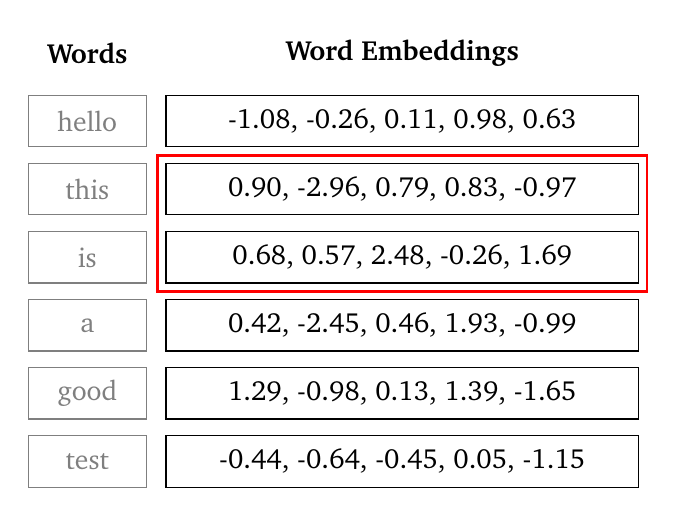
\begin{tikzpicture}%
\node[black,minimum height=0.65cm] (h1) at (0.0,0.8) {\textbf{Words}};%
\node[black,minimum height=0.65cm] (h2) at (4.0,0.8) {\textbf{Word Embeddings}};%
\node[draw,rectangle,minimum width=1.5cm,black,opacity=0.5,align=center,minimum height=0.65cm,below=0.2cm of h1] (0) {hello};%
\node[draw,rectangle,minimum width=6cm,black,align=center,minimum height=0.65cm,below=0.2cm of h2] (vec_0) {-1.08,  -0.26,  0.11,  0.98,  0.63};%
\node[draw,rectangle,minimum width=1.5cm,black,opacity=0.5,align=center,minimum height=0.65cm,below=0.2cm of 0] (1) {this};%
\node[draw,rectangle,minimum width=6cm,black,align=center,minimum height=0.65cm,below=0.2cm of vec_0] (vec_1) {0.90,  -2.96,  0.79,  0.83,  -0.97};%
\node[draw,rectangle,minimum width=1.5cm,black,opacity=0.5,align=center,minimum height=0.65cm,below=0.2cm of 1] (2) {is};%
\node[draw,rectangle,minimum width=6cm,black,align=center,minimum height=0.65cm,below=0.2cm of vec_1] (vec_2) {0.68,  0.57,  2.48,  -0.26,  1.69};%
\node[draw,rectangle,minimum width=1.5cm,black,opacity=0.5,align=center,minimum height=0.65cm,below=0.2cm of 2] (3) {a};%
\node[draw,rectangle,minimum width=6cm,black,align=center,minimum height=0.65cm,below=0.2cm of vec_2] (vec_3) {0.42,  -2.45,  0.46,  1.93,  -0.99};%
\node[draw,rectangle,minimum width=1.5cm,black,opacity=0.5,align=center,minimum height=0.65cm,below=0.2cm of 3] (4) {good};%
\node[draw,rectangle,minimum width=6cm,black,align=center,minimum height=0.65cm,below=0.2cm of vec_3] (vec_4) {1.29,  -0.98,  0.13,  1.39,  -1.65};%
\node[draw,rectangle,minimum width=1.5cm,black,opacity=0.5,align=center,minimum height=0.65cm,below=0.2cm of 4] (5) {test};%
\node[draw,rectangle,minimum width=6cm,black,align=center,minimum height=0.65cm,below=0.2cm of vec_4] (vec_5) {-0.44,  -0.64,  -0.45,  0.05,  -1.15};%
\node[draw,red,fit=(vec_1) (vec_2),inner sep=0.1cm,line width=1pt] {};%
\end{tikzpicture}%
\caption{Word embeddings for an example sentence}
\end{figure}
\begin{figure}[!ht]
	\centering
	\begin{tikzpicture}
		\tikzstyle{mystyle}=[draw,darkgrey,opacity=0,anchor=east]
		\tikzstyle{level1style}=[draw,minimum height=18pt]
		
		\node[mystyle](l1) at (-3.5, 0.5) {Word};
		\node[mystyle](l1) at (-3.5, -1) {Tokens};
		
		\draw
			node[rectangle,draw,line width=1pt,fill=lightgrey](word) at (-0.5,0.5) {university}
			node[level1style](n1) at (-2, -1) {uni}
			node[level1style](n2) at (-1, -1) {niv}		
			node[level1style](n3) at (0, -1) {...}
			node	[level1style](n4) at (1, -1) {ity};
		
		\coordinate[above=0.25cm of n1](c1);
		\coordinate[above=0.25cm of n2](c2);
		\coordinate[above=0.25cm of n3](c3);
		\coordinate[above=0.25cm of n4](c4);
		
		\draw 
			(n1.north) -- (c1) -| (word.south)
			(n2.north) -- (c2) -| (word.south)
			(n3.north) -- (c3) -| (word.south)
			(n4.north) -- (c4) -| (word.south);
		
	\end{tikzpicture}
	\caption{An example tikz figure showing a diagram}
\end{figure}
%
\begin{figure}[!ht]
	\centering
	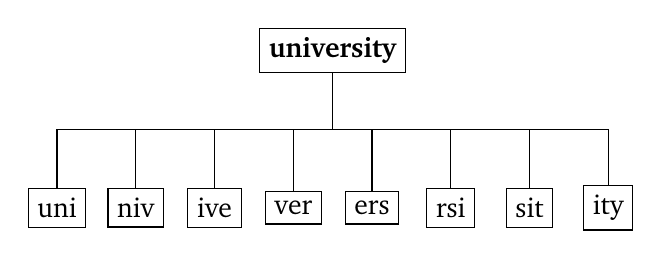
\begin{tikzpicture}
	[
		level 1/.style={level distance=2cm, sibling distance=1cm},
		edge from parent fork down
	]
		\node[draw] {\textbf {university}}
    	child {node[draw] {uni}}
	    child {node[draw] {niv}}
	    child {node[draw] {ive}}
	    child {node[draw] {ver}}
	    child {node[draw] {ers}}
	    child {node[draw] {rsi}}
	    child {node[draw] {sit}}
	    child {node[draw] {ity}};
\end{tikzpicture}
\end{figure}




\newpage


% -------------- START REFERENCES --------------
\bibliography{bibliography/refs}{}
\bibliographystyle{apacite}

% -------------- START APPENDIX --------------
\newpage % TODO: extract to file
\begin{appendices}
\section{Section Heading}
Hello Test
\end{appendices}




\end{document}